\documentclass[xcolor={dvipsnames}]{beamer}
\mode<presentation>
{
  \usetheme{Antibes}      % or try Darmstadt, Madrid, Warsaw, ...
  \usecolortheme{dolphin} % or try albatross, beaver, crane, ...
  \usefonttheme{professionalfonts}  % or try serif, structurebold, ...
  \setbeamertemplate{navigation symbols}{}
  \setbeamertemplate{caption}[numbered]
} 
\usepackage[utf8]{inputenc}
\usepackage[english]{babel}
\usepackage{multirow}
\usepackage{subfigure}
\usepackage{color}
\graphicspath{{/D:/fh/JI/latex/VE230 slides}}
\usepackage{amsmath}
\title[VE230 RC slides week 1]{VE230 RC slides Week 3}
\author{han.fang }
\date{\today}


\begin{document}
\begin{frame}
\titlepage
\end{frame}
\begin{frame}{Overview}
\begin{block}{Content}
	\begin{itemize}
		\item Electrostatics in Free Space
		\item Coulomb’s Law
		\item Gauss’s Law and Application
		\item Electric Potential
	\end{itemize}
\end{block}

\end{frame}
\begin{frame}{Electrostatics in Free Space}
Static electric charges (source) in free space $\rightarrow$ electric field
\begin{block}{Electric field intensity}
\[
\mathbf{E}=\lim _{q \rightarrow 0} \frac{\mathbf{F}}{q} \quad(\mathbf{V} / \mathrm{m})
\]
\end{block}
\end{frame}
\begin{frame}{Fundamental Postulates of Electrostatics}
\begin{itemize}
\item Differential form:
\[
\begin{aligned}
\vec{\nabla \cdot} \mathbf{E}=\frac{\rho}{\epsilon_{0}} \quad (divergence)\\
\vec{\nabla \times} \mathbf{E}=0 \quad (curl)
\end{aligned}
\]
where $\rho$ is the volume charge density of free charges $(C/m^3)$, $\epsilon_0$ is the permittivity of free space, a universal constant.
\item Integral form:
\[
\begin{aligned}
\oint_{S} \mathbf{E} \cdot d \mathbf{s}=\frac{Q}{\epsilon_{0}} \\
\oint_{C} \mathbf{E} \cdot d \ell=0
\end{aligned}
\]
where $Q$ is the total charge contained in volume $V$ bounded by surface $S$. Also, the scalar line integral of the static electric field intensity around any closed path vanishes.
\end{itemize}
\textbf{E} is \textcolor{red}{\textbf{not solenoidal}} (unless $\rho=0$), but \textcolor{red}{\textbf{irrotational}}
\end{frame}
\begin{frame}{Electric Field due to a System of Discrete Charges}
\begin{itemize}
\item \textbf{a single point charge (charge on the origin):}
\[
\mathbf{E}=\mathbf{a}_{R} E_{R}=\mathbf{a}_{R} \frac{q}{4 \pi \epsilon_{0} R^{2}} \quad(\mathbf{V} / \mathbf{m})
\]
\item \textbf{a single point charge (charge is not on the origin):}
\[
\mathbf{E}_{p}=\frac{q\left(\mathbf{R}-\mathbf{R}^{\prime}\right)}{4 \pi \epsilon_{0}\left|\mathbf{R}-\mathbf{R}^{\prime}\right|^{3}} \quad(\mathbf{V} / \mathbf{m})
\]
\begin{figure}[H]
\centering
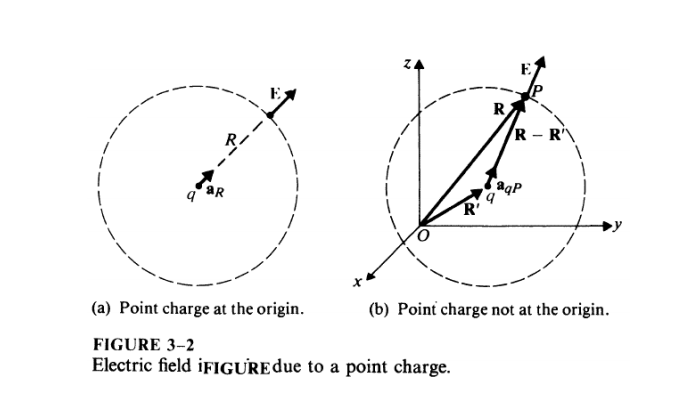
\includegraphics[width=6.5cm]{3_1.png}
\end{figure}
\end{itemize}
\end{frame}
\begin{frame}{Electric Field due to a System of Discrete Charges}
\begin{itemize}
\item \textbf{a single point charge (charge is not on the origin):}
When a point charge $q_2$ is placed in the field of another point charge $q_1$ at the origin, a force $F_{12}$ is experienced by $q_2$ due to the electric field intensity $\vec{E_{12}}$ of $q_1$ at $q_2$. Then we have:
$$\vec{F_{12}} = q_2\vec{E_{12}} = \vec{a_R}\frac{q_1q_2}{4\pi \epsilon_0 R^2}$$
\item \textbf{several point charges:}
\[
\mathbf{E}=\frac{1}{4 \pi \epsilon_{0}} \sum_{k=1}^{n} \frac{q_{k}\left(\mathbf{R}-\mathbf{R}_{k}^{\prime}\right)}{\left|\mathbf{R}-\mathbf{R}_{k}^{\prime}\right|^{3}}
\]
\end{itemize}
\end{frame}
\begin{frame}{Electric Dipole}
\begin{itemize}
\item \textbf{Electric Field}
\begin{figure}[H]
\centering
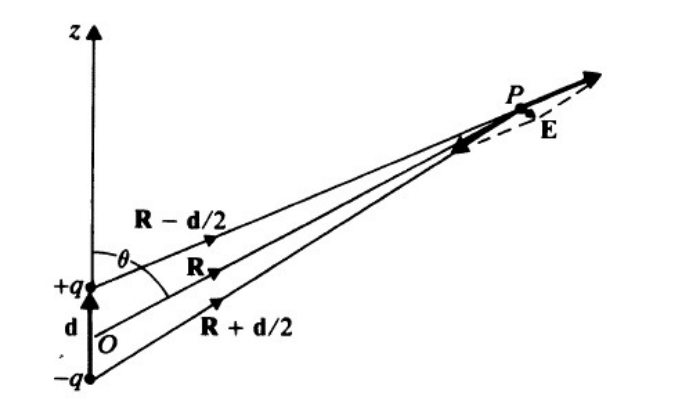
\includegraphics[width=7cm]{3_2.png}
\end{figure}
\end{itemize}
\end{frame}
\begin{frame}{Electric Dipole}
\begin{itemize}
\item \textbf{Electric Field}\\
general expression:
\begin{equation*}
\mathbf{E}=\frac{q}{4 \pi \epsilon_{0}}\left\{\frac{\mathbf{R}-\frac{\mathbf{d}}{2}}{\left|\mathbf{R}-\frac{\mathbf{d}}{2}\right|^{3}}-\frac{\mathbf{R}+\frac{\mathbf{d}}{2}}{\left|\mathbf{R}+\frac{\mathbf{d}}{2}\right|^{3}}\right\}
\end{equation*}
if $d<<R$:
\[
\mathbf{E} \cong \frac{q}{4 \pi \epsilon_{0} R^{3}}\left[3 \frac{\mathbf{R} \cdot \mathbf{d}}{R^{2}} \mathbf{R}-\mathbf{d}\right]
\]

\item \textbf{Electric Dipole Moment}\\
\textbf{Definition:} 
\[
\mathbf{p}=q \mathbf{d}
\]
,where $q$ is the charge, vector $\mathbf{d}$ goes from $-q$ to $+q$.
\[
\begin{aligned}
&\mathbf{p}=\mathbf{a}_{z} p=p\left(\mathbf{a}_{R} \cos \theta-\mathbf{a}_{\theta} \sin \theta\right)\\
&\mathbf{R} \cdot \mathbf{p}=R p \cos \theta\\
\end{aligned}
\]
\end{itemize}
\end{frame}
\begin{frame}{Electric Dipole}
\begin{itemize}
\item \textbf{Electric Field:} (spherical coordinate)
\[
\mathbf{E}=\frac{p}{4 \pi \epsilon_{0}R^{3}}\left(\mathbf{a}_{R} 2 \cos \theta+\mathbf{a}_{\theta} \sin \theta\right) \quad(\mathrm{V} / \mathrm{m})
\]
\end{itemize}
\end{frame}
\begin{frame}{Electric Field due to a Continuous Distribution of Charge}
\begin{itemize}
\item \textbf{General Differential Element:}
\[
d \mathbf{E}=\mathbf{a}_{R} \frac{\rho d v^{\prime}}{4 \pi \epsilon_{0} R^{2}},
\]
where $dv^\prime$ is the differential volume element.  

\item \textbf{Line Charge:}
\[
\mathbf{E}=\frac{1}{4 \pi \epsilon_{0}} \int_{L^{\prime}} \mathbf{a}_{R} \frac{\rho_{\ell}}{R^{2}} d \ell^{\prime} \quad(\mathbf{V} / \mathbf{m})
\]
\item \textbf{Surface Charge:}
\[
\mathbf{E}=\frac{1}{4 \pi \epsilon_{0}} \int_{\mathbf{S}^{\prime}} \mathbf{a}_{R} \frac{\rho_{s}}{R^{2}} d s^{\prime} \quad(\mathbf{V} / \mathrm{m})
\]
\item \textbf{Volume Charge:}
\[
\mathbf{E}=\frac{1}{4 \pi \epsilon_{0}} \int_{V^{\prime}} \mathbf{a}_{R} \frac{\rho}{R^{2}} d v^{\prime} \quad(\mathbf{V} / \mathbf{m})
\]
\end{itemize}
\end{frame}
\begin{frame}{Gauss’s Law and Application}
\begin{block}{Definition}
The total outward flux of the E-field over any closed surface in free space is equal to \textbf{the total charge enclosed in the surface} divided by $\epsilon_0$. (Note that we can choose arbitrary surface $S$ for our convenience.)
\[
\oint_{S} \mathbf{E} \cdot d \mathbf{s}=\frac{Q}{\epsilon_{0}}
\]
\end{block}
\begin{block}{Application}
\begin{itemize}
\item \textbf{Conditions for Maxwell's Integral Equations:}\\
There is \textcolor{red}{\textbf{a high degree of symmetry}} in the charge distribution or in the electrical field (i.e., spherically symmetric, planar, line charge, etc.
\end{itemize}
\end{block}

\end{frame}
\begin{frame}{Gauss’s Law Application}
\begin{block}{\textbf{Example:}}
Determine the electric field intensity of an infinitely long, straight, line charge of a uniform density $\rho_s$ in air.
\end{block}
\pause
\begin{block}{Answer}
$$E\cdot 2\pi \cdot r \cdot l = \frac{\rho \cdot l}{\epsilon_0}$$
\end{block}
\end{frame}
\begin{frame}{Several Useful Models}
\textbf{Note:} The charge distribution should be \textcolor{red}{\textbf{uniform}}.
\begin{table}[H]
  \centering
    \begin{tabular}{cc}
      \hline
   different models & E(magnitude)\\ \hline
    infinitely long, line charge &$E=\frac{ \rho_{\ell}}{ 2\pi r \epsilon_0} $ \\   \hline
    infinite planar charge &  $E=\frac{\rho_s}{2\epsilon_0}$\\   \hline
    uniform spherical surface charge with radius R & $\left\{\begin{array}{l}E=0(r<R) \\ E=\frac{Q}{4\pi r^2 \epsilon_0} (r>R)\end{array}\right.$ \\   \hline
    uniform sphere charge with radius R & $\left\{\begin{array}{l}E=\frac{Qr}{4\pi R^3}(r<R) \\ E=\frac{Q}{4\pi r^2 \epsilon_0} (r>R)\end{array}\right.$ \\   \hline
    infinitely long, cylindrical charge with radius R & $\left\{\begin{array}{l}E=\frac{\rho_v r}{2\epsilon_0}(r<R) \\ E=\frac{\rho_v R^2}{2r\epsilon_0} (r>R)\end{array}\right.$ \\   \hline
    \end{tabular}%
  \label{tab:addlabel}%
\end{table}%
\end{frame}
\begin{frame}{Electric Potential}
\begin{itemize}
\item \textbf{Expression:}
\[
\mathbf{E}=-\nabla V
\]
the reason for the negative sign: consistent with the convention that in going against the $\mathbf{E}$ field, the electric potential $V$ increases.

\item \textbf{Electric Potential Difference:}
\[
V_{2}-V_{1}=-\int_{P_{1}}^{P_{2}} \mathbf{E} \cdot dl
\]
\item \textbf{Electric Potential due to a Charge Distribution}

$$V = \frac{q}{4\pi \epsilon_0 R}$$
\end{itemize}
\end{frame}
\begin{frame}{Electric Potential}
\begin{itemize}
\item \textbf{Line Charge:}
\[
V=\frac{1}{4 \pi \epsilon_{0}} \int_{L^{\prime}} \frac{\rho_{l}}{R} dl^{\prime} \quad(V)
\]
\item \textbf{Surface Charge:}
\[
V=\frac{1}{4 \pi \epsilon_{0}} \int_{\mathbf{S}^{\prime}}  \frac{\rho_{s}}{{R}} d s^{\prime} \quad(V)
\]
\item \textbf{Volume Charge:}
\[
V=\frac{1}{4 \pi \epsilon_{0}} \int_{V^{\prime}} \frac{\rho}{R} d v^{\prime} \quad(V)
\]
\end{itemize}
\end{frame}
\begin{frame}{Assignment}
\begin{block}{P.3-22}
The polarization in a dielectric cube of side L centered at the origin is given by $\mathbf{P}=P_0(\mathbf{a_x}x+\mathbf{a_y}y+\mathbf{a_z}z)$.\\
\textbf{a)} Determine the surface and volume bound-charge densities\\
\textbf{b)} Show that the total bound charge is zero.\\

\end{block}
\pause
\begin{figure}[H]
	\centering
	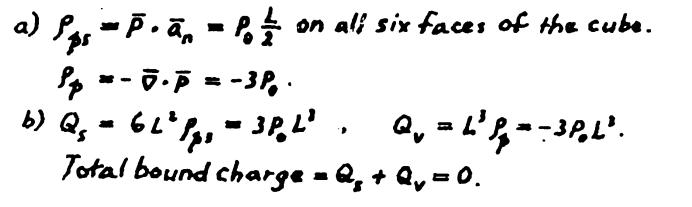
\includegraphics[width=0.9\linewidth]{3_3.png}
\end{figure}
\end{frame}
\begin{frame}{Assignment}
\begin{block}{P.3-23}
Determine the electric field intensity at the center of a small spherical cavity cut out of a large block of dielectric in which a polarization \textbf{P} exists.

\end{block}
\pause
\begin{figure}[H]
	\centering
	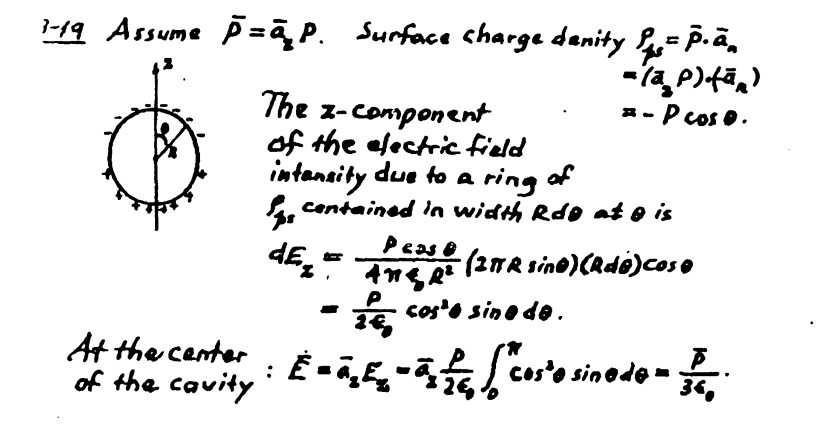
\includegraphics[width=0.8\linewidth]{3_4.png}
\end{figure}
\end{frame}
\begin{frame}{Assignment}
\begin{block}{P.3-25}
Assume that the z=0 plane separates two lossless dielectric regions with $\epsilon_{r1}=2$ and $\epsilon_{r2}=3$. If we know that $\boldsymbol{E_1}$ in region 1 is $\boldsymbol{a_x}2y-\boldsymbol{a_y}3x+\boldsymbol{a_z}(5+z)$, what do we also know about $\boldsymbol{E_2}$ and $\boldsymbol{D_2}$ in region 2? Can we determine $\boldsymbol{E_2}$ and $\boldsymbol{D_2}$ at any point in region 2? Explain.\\
\end{block}
\pause
\begin{figure}[H]
	\centering
	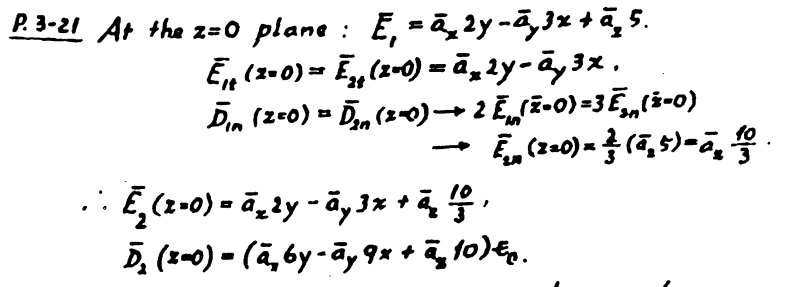
\includegraphics[width=0.8\linewidth]{3_5.png}
\end{figure}
\end{frame}
\begin{frame}{Assignment}
\begin{block}{P.3-28}
Dielectric lenses can be used to collimate electromagnetic fields. In Fig.1 the left surface of the lens is that of a circular cylinder, and the right surface is a plane. If $\boldsymbol{E_1}$ at point $P(r_0,45^{\circ},z)$ in region 1 is $\boldsymbol{a_r}5-\boldsymbol{a_{\phi}}3$, what must be the dielectric constant of the lens in order that $\boldsymbol{E_3}$ in region 3 is parallel to the x-axis?\\
\end{block}
\begin{figure}[H]
	\centering
	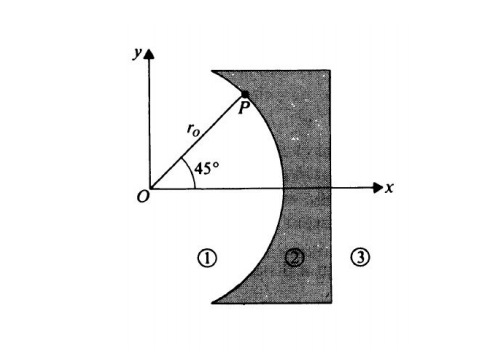
\includegraphics[width=0.6\linewidth]{3_6.png}
\end{figure}
\end{frame}
\begin{frame}{Assignment}
\begin{figure}[H]
	\centering
	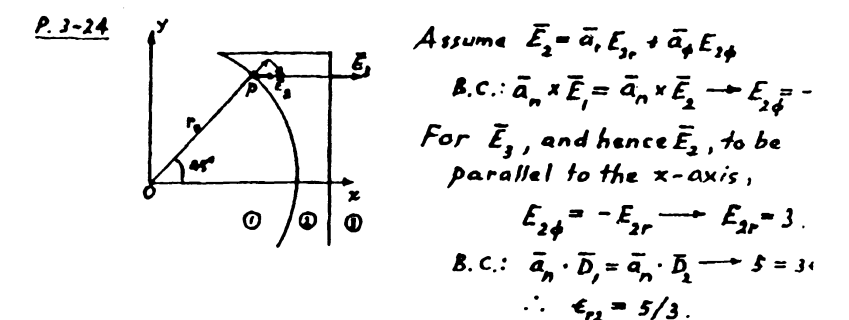
\includegraphics[width=0.98\linewidth]{3_7.png}
\end{figure}
\end{frame}
\begin{frame}{Assignment}
\begin{block}{P.3-32}
The radius of the core and the inner radius of the outer conductor of a very long coaxial transmission line are $r_i$ and $r_o$, respectively. The space between the conductors is filled with two coaxial layers of dielectrics. The dielectric constants of the dielectrics are $\epsilon_{r_1}$ for $r_i<r<b$ and $\epsilon_{r2}$ for $b<r<r_o$. Determine its capacitance per unit length.\\
\end{block}
\pause
\begin{figure}[H]
	\centering
	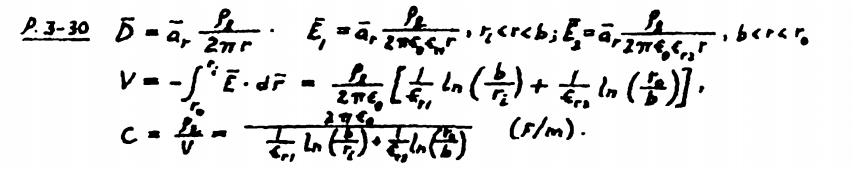
\includegraphics[width=0.95\linewidth]{3_8.png}
\end{figure}
\end{frame}
\end{document}